\documentclass{article} % For LaTeX2e
\usepackage{nips15submit_e}
\usepackage{hyperref}
\usepackage{url}
\usepackage{float}
\usepackage{graphicx}
\usepackage{caption}
\usepackage{subcaption}
\usepackage{capt-of}
%\documentstyle[nips14submit_09,times,art10]{article} % For LaTeX 2.09


\title{Making Music with Hidden Markov Models}


\author{
Anna Yanchenko \\
Duke University\\
\texttt{anna.yanchenko@duke.edu} \\
\And
Megan Robertson \\
Duke University \\
\texttt{megan.robertson@duke.edu} \\
}


\newcommand{\fix}{\marginpar{FIX}}
\newcommand{\new}{\marginpar{NEW}}

\nipsfinalcopy % Uncomment for camera-ready version

\begin{document}


\maketitle

\begin{abstract}
We use Hidden Markov Models (HMM) to capture the latent elements involved in music creation. The observed states are the notes and velocity, volumes, of each note. The latent states include elements such as chord progression, dynamics and patterns.In this paper, we implement three different Hidden Markov Models and compare the resulting compositions for each model. These models are trained on various classical piano pieces, and the resulting compositions are compared.
\end{abstract}
 
\section{Introduction}

Hidden Markov Models are known for their use in language applications such as speech recognition and handwriting recognition programs. However, it is also possible to use Hidden Markov Models in another language application, the language of music. This project serves as a platform to combine our shared interests of music and statistics. 

The project uses music data in the form of  Musical Instrument Digital Interface (MIDI) files. This interface creates a form of communication between computers and musical instruments that enables them to send instructions back and forth. MIDI files can contain multiple channels that store information about the notes and velocity of certain instruments. The files also contain information about when a particular note starts and stops. \footnote{MIDI Manufacturers Association, "An Introduction to MIDI"}. 

Any musician or student of music can tell you that there is more to composing music beyond stringing together some notes with a catchy rhtyhm. There are many things to consider such as chord progression, dynamics, and patterns. It is importnat for a composer to be fmant for a composer to be familar with things such as the Circle of Fifths. There are also different forms, sonata, rondo, blues and more, that can be used in the creation of music.\footnote{Music Composition for Dummies, \url{http://www.dummies.com/how-to/content/music-composition-for-dummies-cheat-sheet.html}}

However, the MIDI data does not capture all of the theory and ideas that create a composition. Therefore, we use Hidden Markov Models (HMMs) in order to capture both the observed states, the note/velocity information, as well as the latent variables, theory such as that described above. We utitilze three different HMMs and train them on classical piano pieces. The estimated parameters are then used to compose new pieces.


\section{Methods}

Classical piano pieces were used to train each of the models. In this paper we present the result forGustav Holt's Jupiter from "The Planets" and Johann Pachelbel's Canon. A piano arrangement of Jupiter was used as opposed to the orchestral piece. The MIDI files for these songs were converted to Comma Separated Value (CSV) files.\footnote{This was done using a program found at \url{http://www.fourmilab.ch/webtools/midicsv/}} 

The classical pieces were used to estimate the respective parameters of the models described below. In this training, the tempo, key signature and length of the original song were not changed. The only possible observed states were the velocities and notes present in the original pieces. Once the parameters had been estimated, they were used to generate a new piece of music. This process generates a CSV file of the new composition, and this file is then converted to a MIDI file using the same program as above. The files can then be played on a synsthesizer or a program such as GarageBand.

The three models used are described in the subsections below. They are a first order HMM, a second order HMM, and a first order HMM with two hidden states. In order to evaluate the performance of each model, twenty-two survey respondents determined which of the compositions they liked best for either Pachabel's Cannon or Holst's Jupiter. They also were provided with both the original Jupier and Cannon, and asked which of the original versions they thought inspired the remixes. 

\subsection {Model 1: First Order Hidden Markov Model}

The simplest of the three models is the first order Hidden Markov Model. In this model, the observed values, $X_i$, are the notes and their velocity. The model has only one hidden state for each note/velocity pair, $Z_i$, and each hidden state only depends on the prior hidden state. 

\begin{figure}[H]
\centering
\caption{Graphical Model - First Order HMM}
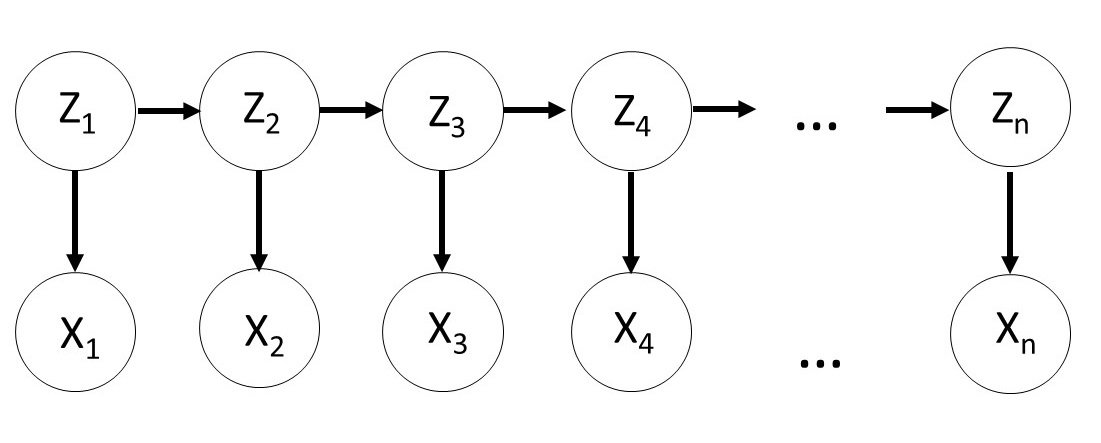
\includegraphics [scale = 0.35] {Model1.jpg}
\end{figure}

The Baum-Welch Alogirithm was used to estimate the parameters of this model. For details of the derivations and algorithm see class notes. \footnote{Statistics 531, Duke University Spring 2016. Instructor: Jeff Miller}
 
\subsection{Model 2: Second Order Hidden Markov Model}

The second model expanded on Model 1 by assuming that each state also depended on the prior two states. This enables the model to capture the structure that is evolving over time in the piece. The Baum-Welch Algorithm was again used to estimate the parameters. The details of the algorithm for this model can be found in Mari and Schott's "Probabilistic and Statsitical Methods in Computer Science." \footnote{Jean-Francoix Mari and Rene Schott, "Probabilistic and Statistical Methods in Computer Science", Springer Science, pg. 161-167 and Brett Watson and Ah Chung Tsoi, "Second Order Hidden Markov Models for Speech Recognition", Univsersity of Queensland}.

\begin{figure}[H]
\centering
\caption{Graphical Model - Second Order HMM}
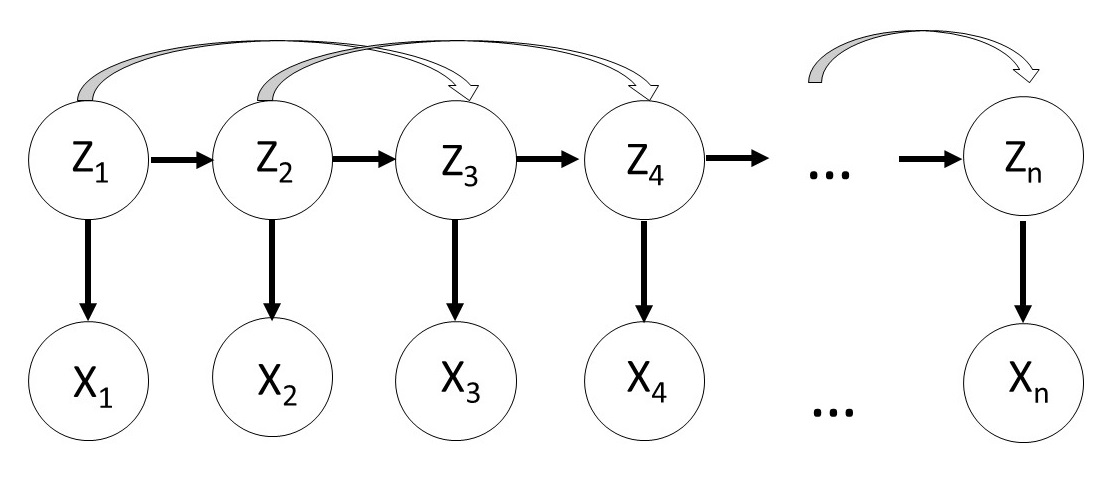
\includegraphics [scale = 0.35] {Model2.jpg}
\end{figure}

\subsection{Model 3: HMM with Two Hidden States}

The final model expanded on the intital model by adding a second latent variable. This meta-state allows the model to capture additional aspects of the hidden states and the music generation process.  This processes might evolve at a rate different than the processes that are present in the observed states and one latent state. 

\begin{figure}[H]
\centering
\caption{Graphical Model - First Order HMM with Two Hidden States}
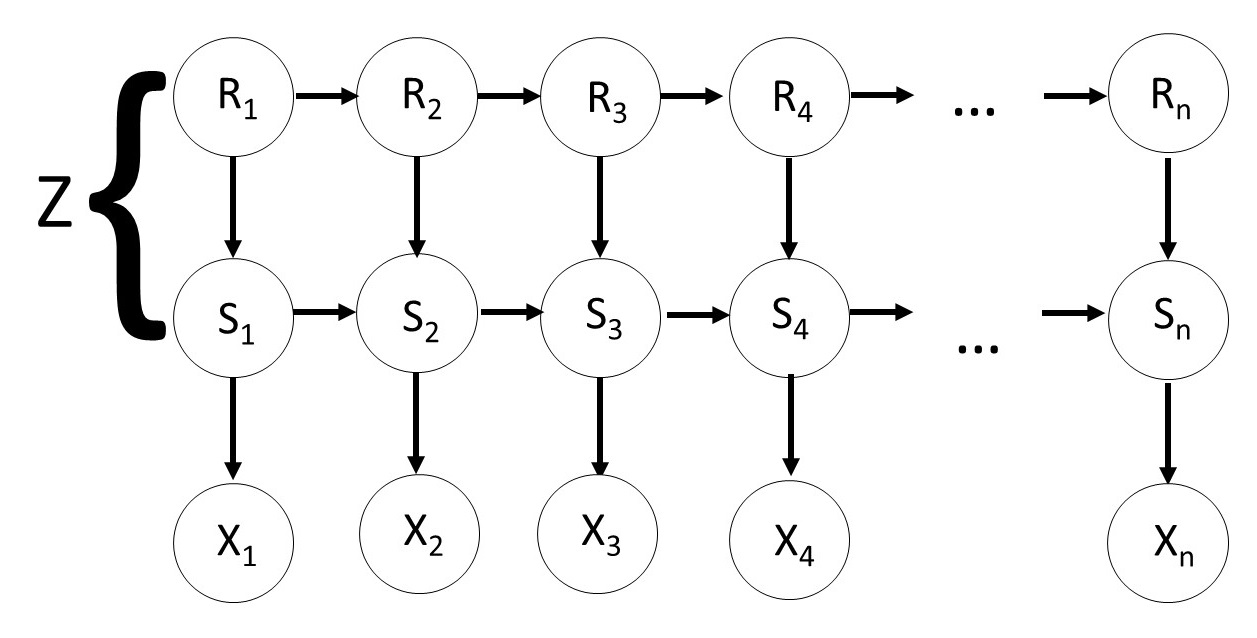
\includegraphics [scale = 0.35] {Model3.jpg}
\end{figure}

For the derivation of the Baum-Welch algorithm for this model, see the Appendix.

\section{Results}

\subsection{Original Pieces}

Of the four pieces used to train the various models, Jupiter and Pachabel's Cannon provided the best results. It is possible that these pieces performed the best because of their prominent melody from the beginning. For example, in Claude Debussy's Clair de Lune, the piece builds for a while before the melody emerges. Our models may not have worked well for this because they did not have the capability to capture the building structure and melody of the song. 

\begin{figure}[H]
\centering
\caption{Jupiter - Original Song}
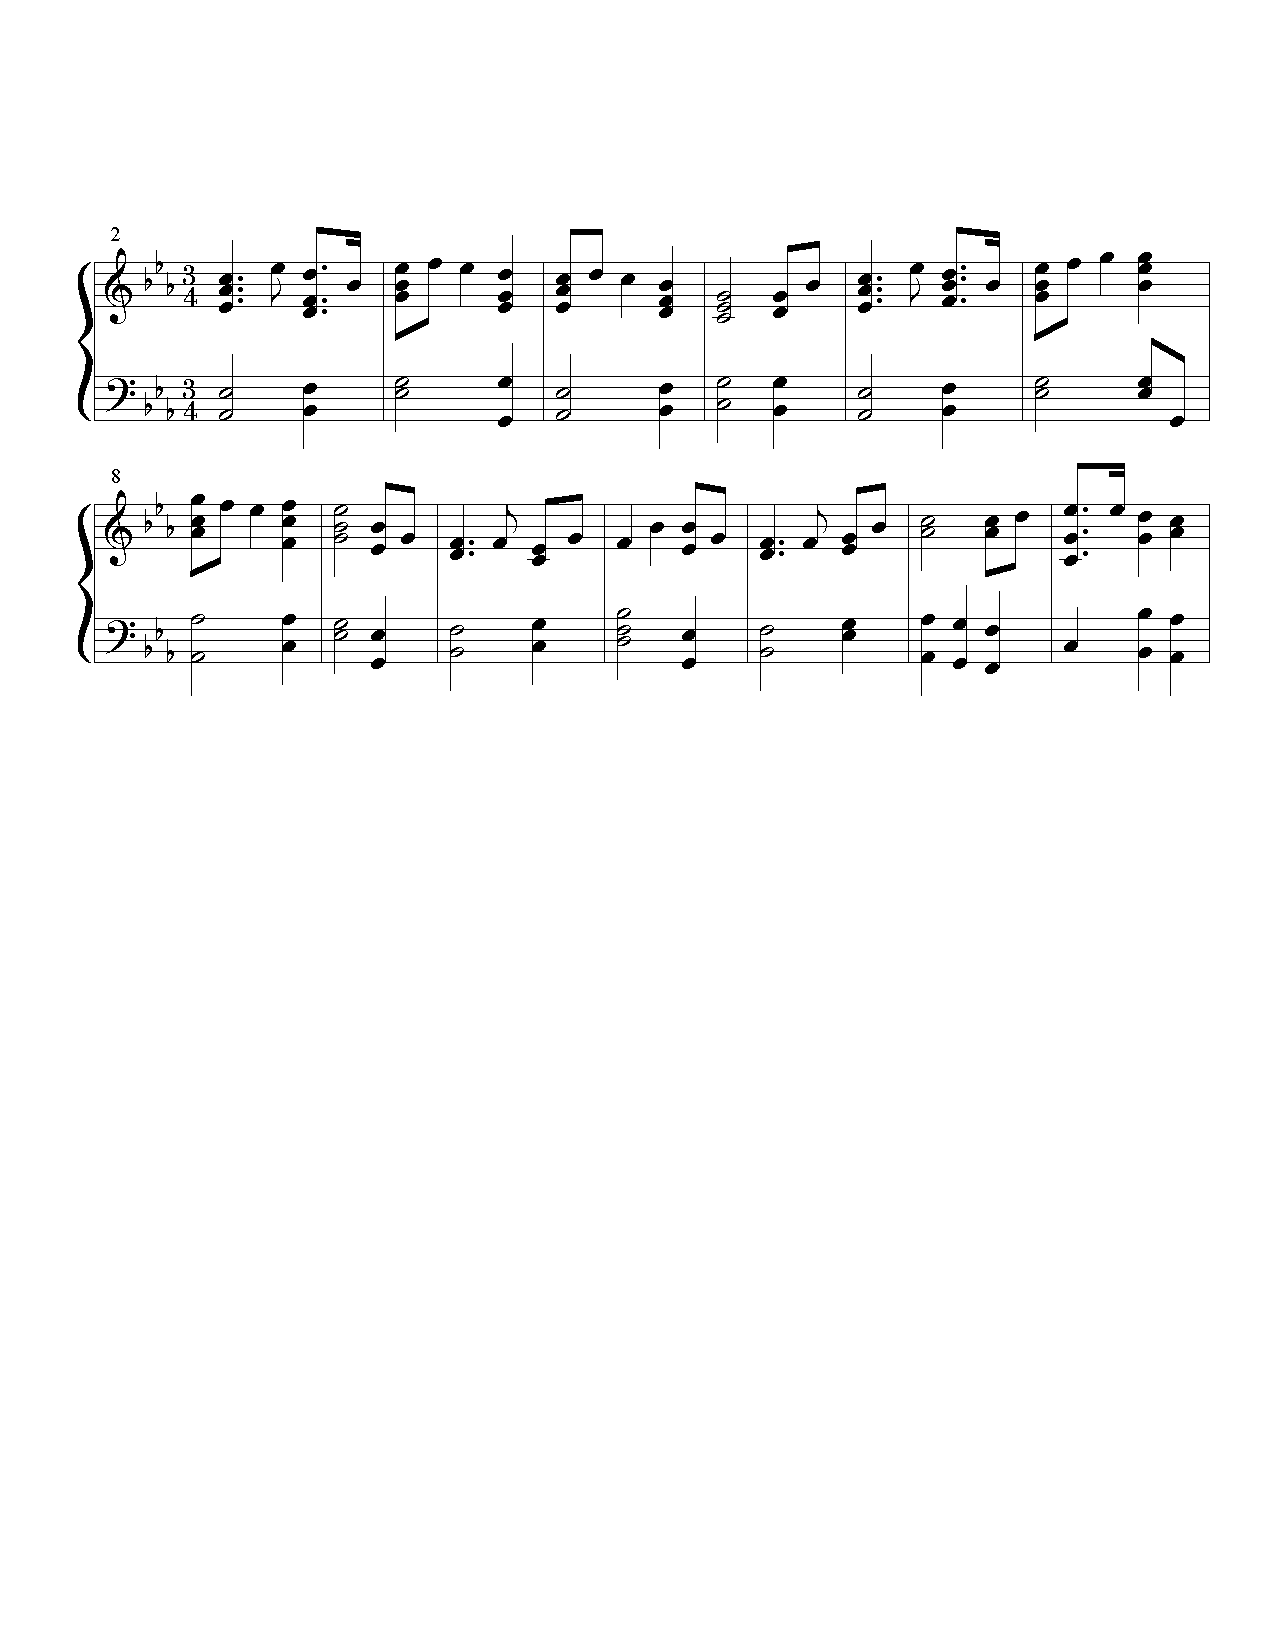
\includegraphics [scale = 0.6] {JupiterOriginal-cropped.pdf}
\end{figure}

Both Jupiter and Pachabel's Cannon are well-known classical pieces whose themes occur frequently in advertisements and other media forms. The two pieces have a logical progression. It is obvious that these pieces are structurally sound and musically cohesive given their notoriety. 

\subsection{First Order Hidden Markov Model}

The Jupiter remix created using the first order Hidden Markov Model had lots of octave and interval jumps that were not present in the original song. For example, this behavior can be seen in measures one, three and four. In additoin, there are more rests in the first two lines of the remix and there are also more quarter and half notes. The melody of the song seems to be distributed about equally between the left and the right hands. The left hand controlled most of the melody in the original composition. There is also no resolution in the remix.

\begin{figure}[H]
\centering
\caption{Jupiter Remix - Model 1}
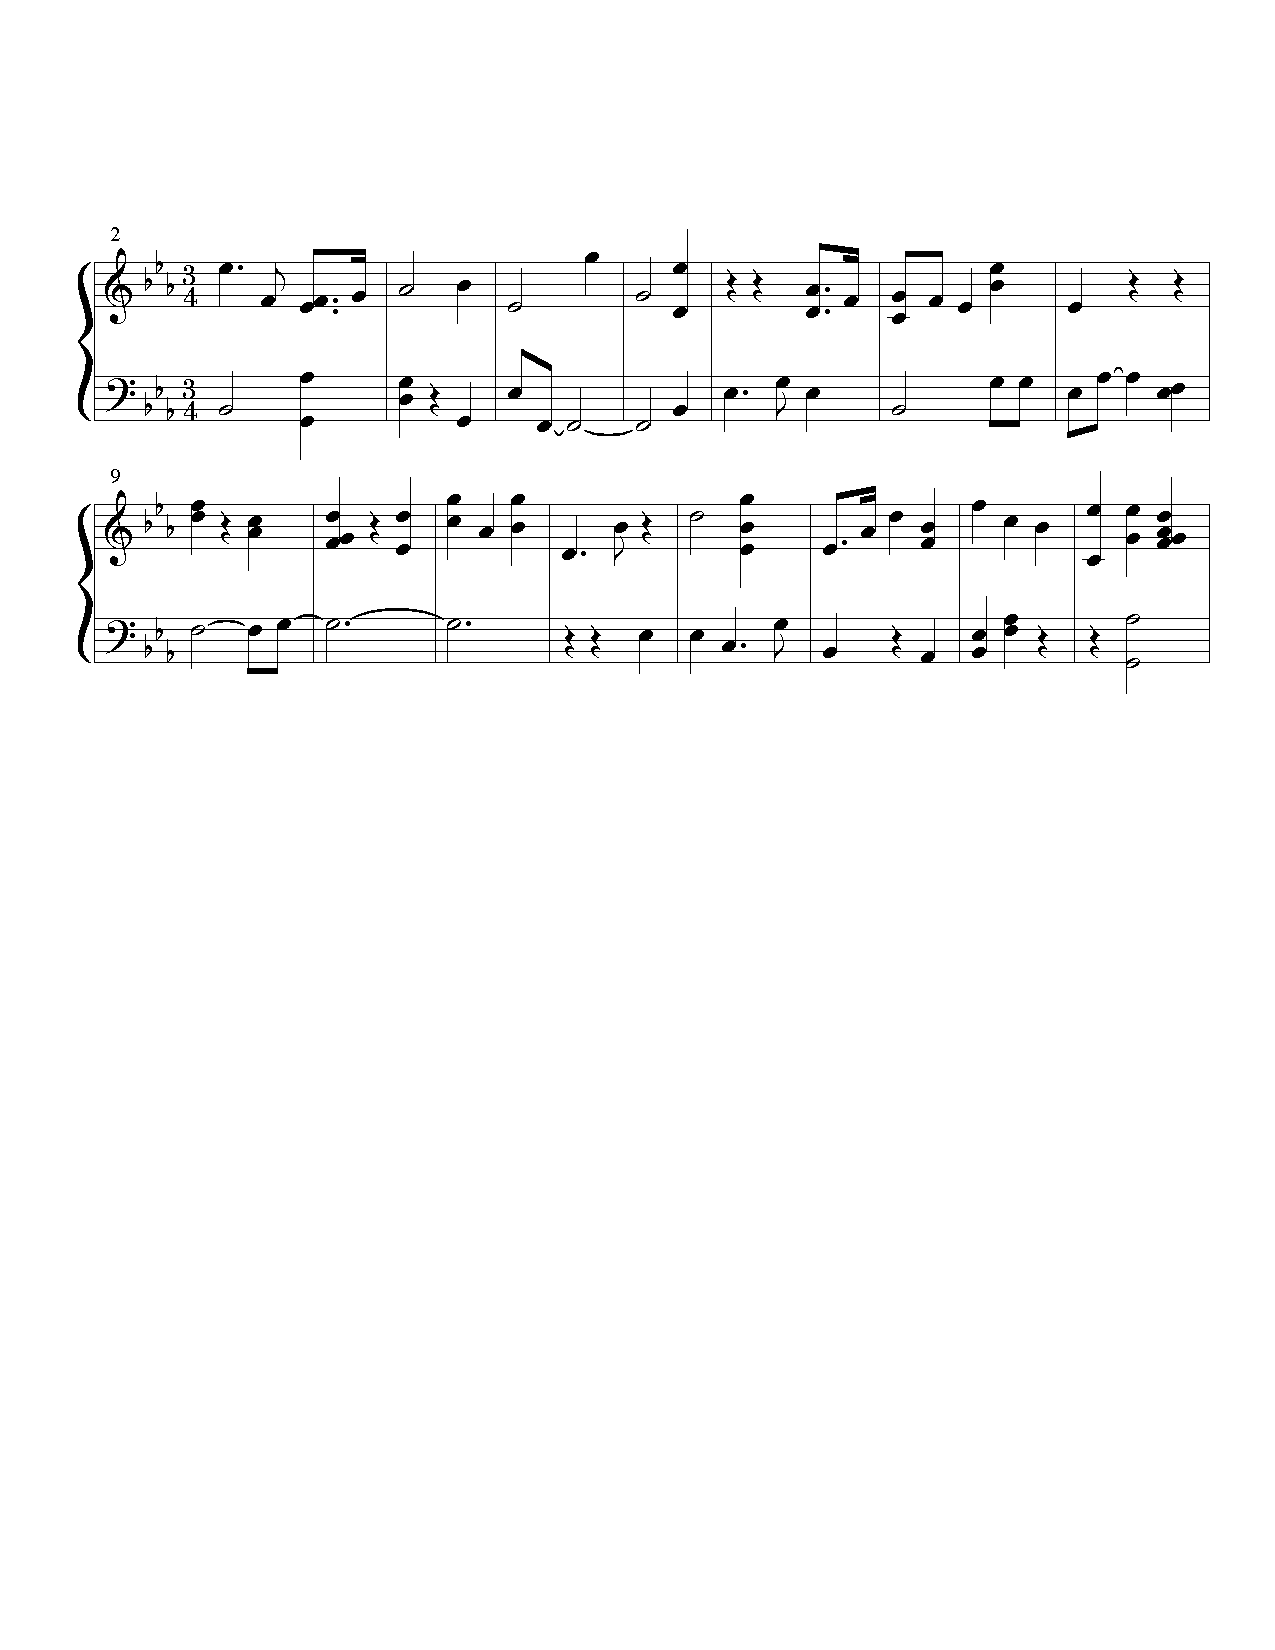
\includegraphics [scale = 0.6] {JupiterRemix-cropped.pdf}
\end{figure}

The remixed version of Pachabel's Cannon has less sixteenth notes but more dotted notes. Pachabel's Cannon consists of mostly eighth or sixteenth notes for the melody. There are also more rests in this remixed version than there are in the original. Finally, there are large octave jumps and jumps of large intervals in this version.

The first order HMM compositions sounded very different from the original compositions. This probably occurs because the model does not capture enough of the overall structure. Thus there are some notes that occur together and should not. For example, the melody for Pachabel's cannon builds over several measures. The first order HMM only has the state depend on the former state. A model that captured more structure could have the potential to incorporate the whole chord from the previous state. 

\subsection{Second Order Hidden Markov Model}

The Juptier composition created using the second order Hidden Markov Model is an improvement on the first remix. It still has some large interval jumps, but fewer jumps than that from Model 1. The chords also make more sense in the piece, but there is less dissonance. The piece also has fewer rests than the first order composition, but more rests than i nthe original composition.


\begin{figure}[H]
\centering
\caption{Jupiter Remix - Model 2}
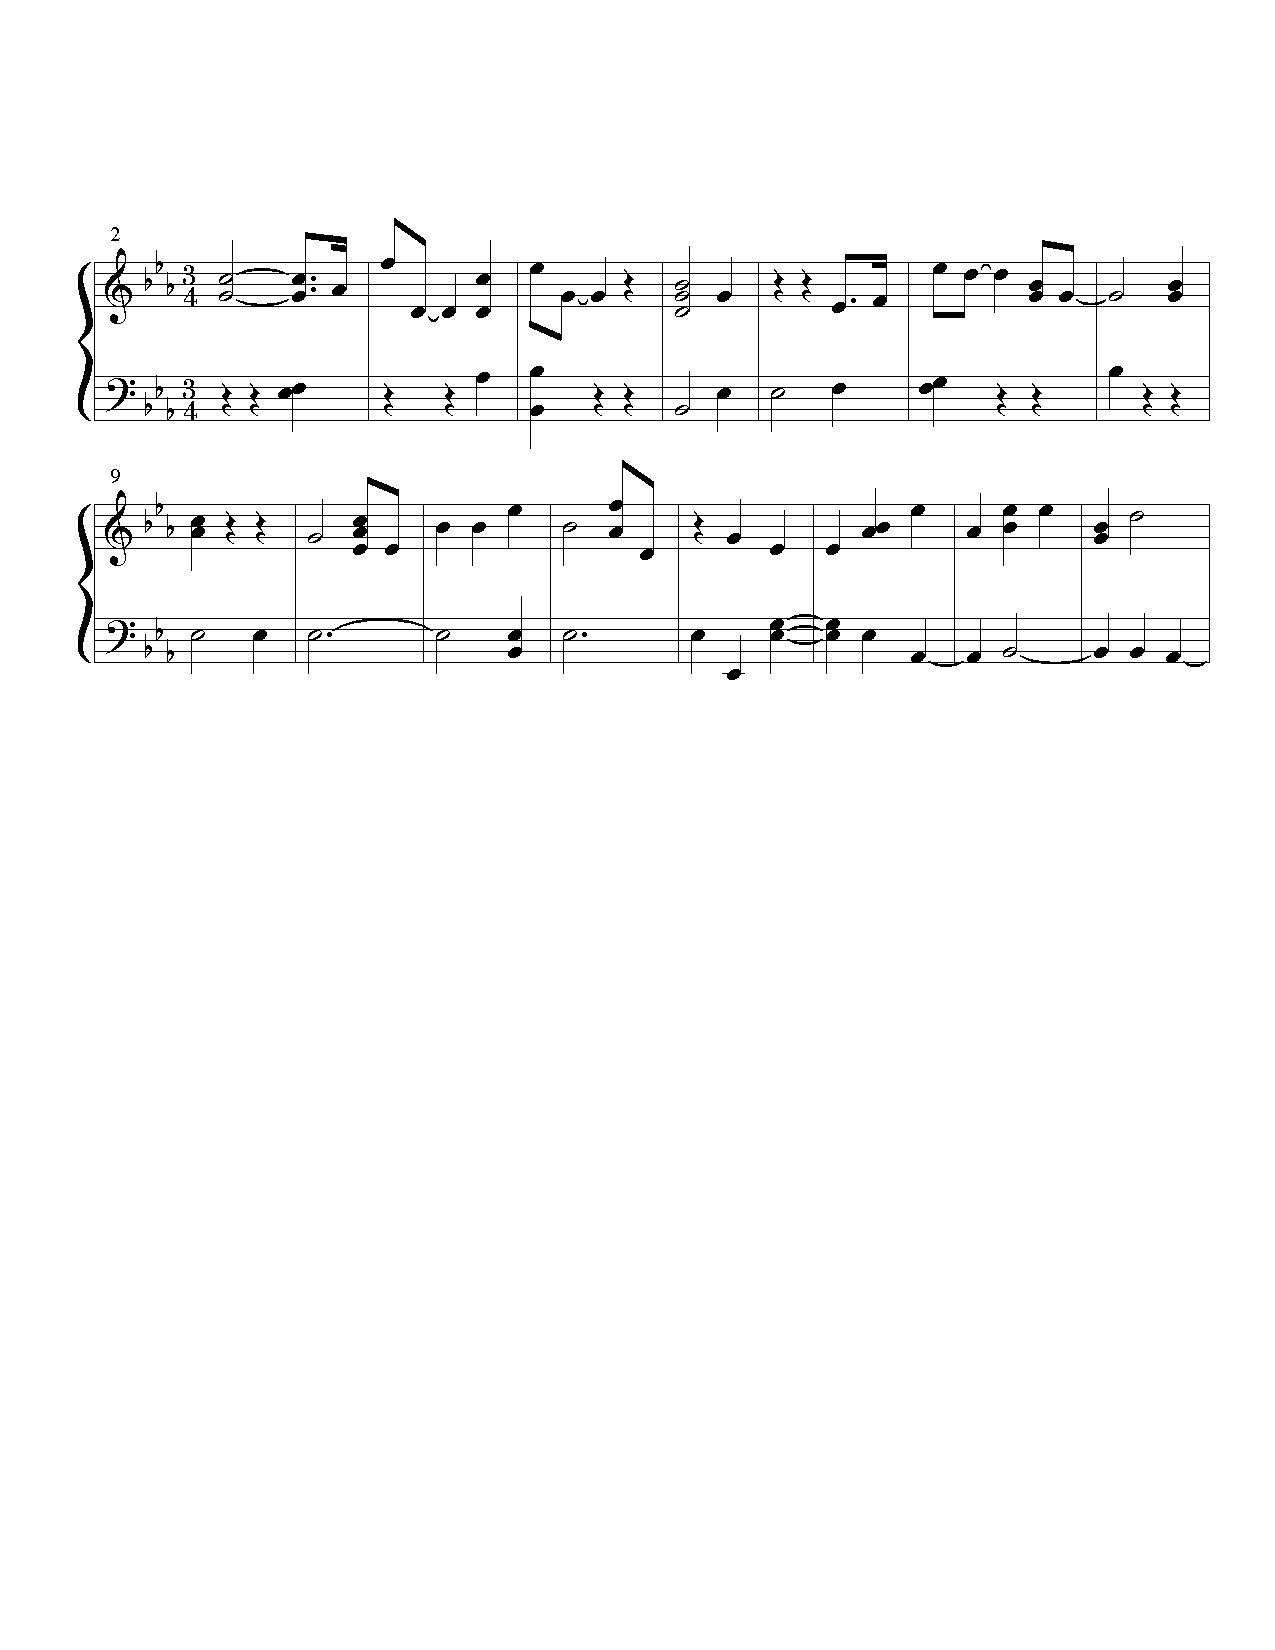
\includegraphics [scale = 0.6] {JupiterRemix2-cropped.pdf}
\end{figure}

The Cannon composition created using the second order Hidden Markov Model has more sixteenth notes than the first remix, but fewer sixteenth notes than the original version. There are still awkward interval jumps present in the piece. Overall, the chords made more sense and there was less dissonance in this piece than the first remix. The progression of the song seemed to be more logical than the first model. This probably occured because the second order HMM captures more structure than the first order HMM.

\subsection{First Order Hidden Markov Model with Two Hidden States}

OF the three remixes, this version had the fewest rests of the remixed compositions, but more than the original version. It also contained large interval jumps. These jumps between notes were larger than the noes that occured in the original song, but were smaller than the jumps in the other versions. 


\begin{figure}[H]
\centering
\caption{Jupiter Remix - Model 2}
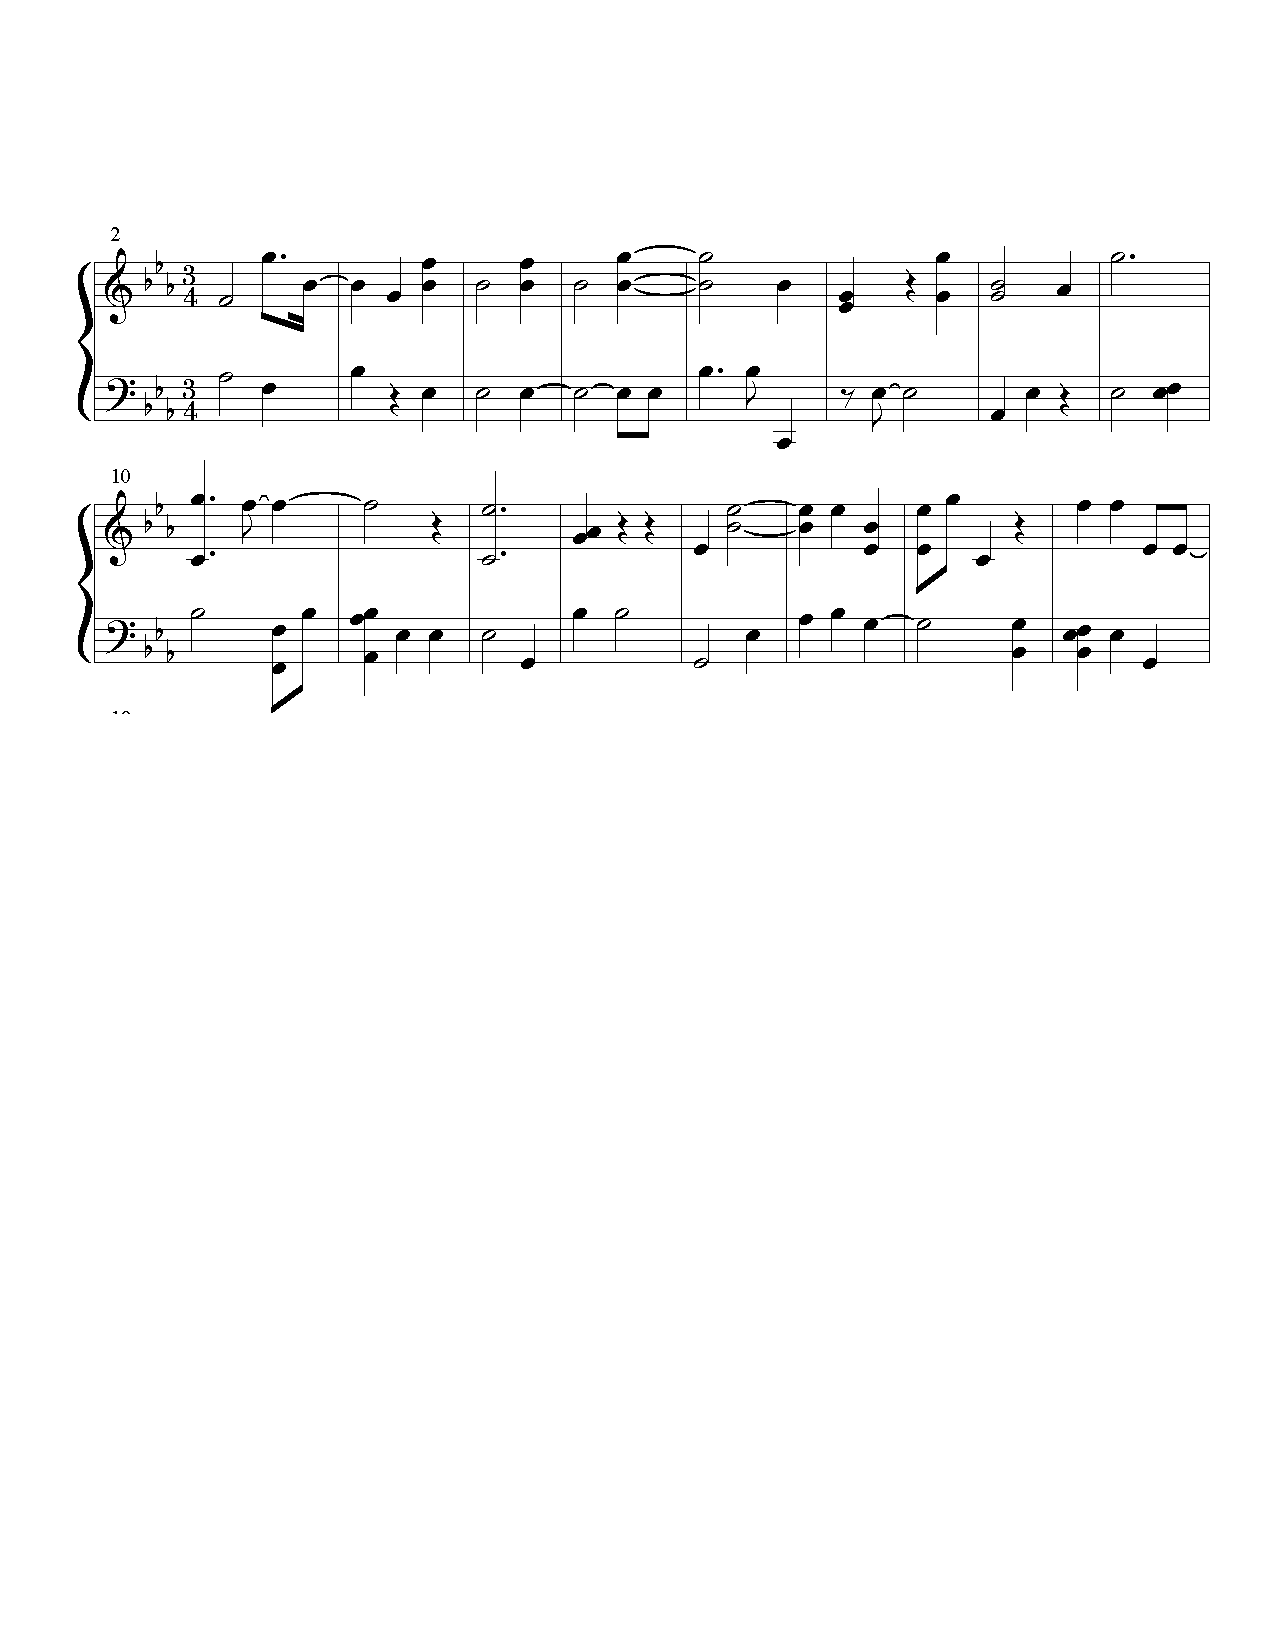
\includegraphics [scale = 0.6] {JupiterRemix2H-cropped.pdf}
\end{figure}

The two latent state version had more eighth and sixteenth notes than the other two remix versions. However, it still did not have as many as the original version. There are still large jumps in between notes. 


\subsection{Summary}
Overall, the remix created using the second order Hidden Markov Model appeared to have the best structure of all of the remixes. On the other hand, the remix created using the first order Hidden Markov Model with two latent states had better chords. In all of the new compositions, the melody seemed to be split between the two hands. The models did not catch the general structure that lower notes, those played by the right hand, were longer in the original versions of the pieces. Most of melody was in the right hand notes. In all of the models, the dynamics were modeled independently and as a result the dynamics did always occur in a logical fashion. There are many instances where certain notes are uncomfortably loud compared to the rest of the piece. 

Figure eight displays the results of the survey. Of the listeners asked about the compositions inspired by Pachabel's Cannon, three preferred Model 1, six preferred Model 2 and only one preferred Model 3. Six out of ten correctly identified the original compositon. On the other hand, eight of twelve respondents correctly chose Jupiter as the original composition for the other remixes. None of the resondents preferred Model 1, ten preferred Model 2 and two preferred Model 3. For both groups, Model 2 was the overall preferred composition. 




\begin{figure}
\centering
\begin{subfigure}{.5\textwidth}
  \centering
  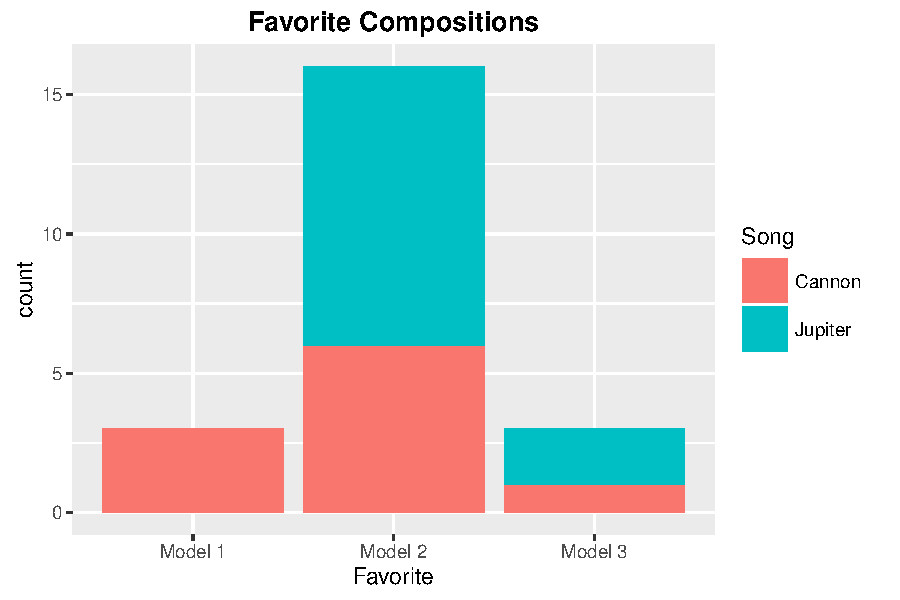
\includegraphics[scale = 0.5]{SurveyFav.pdf}
  \caption{Preferred Compositions}
  \label{fig:sub1}
\end{subfigure}%
\begin{subfigure}{.5\textwidth}
  \centering
  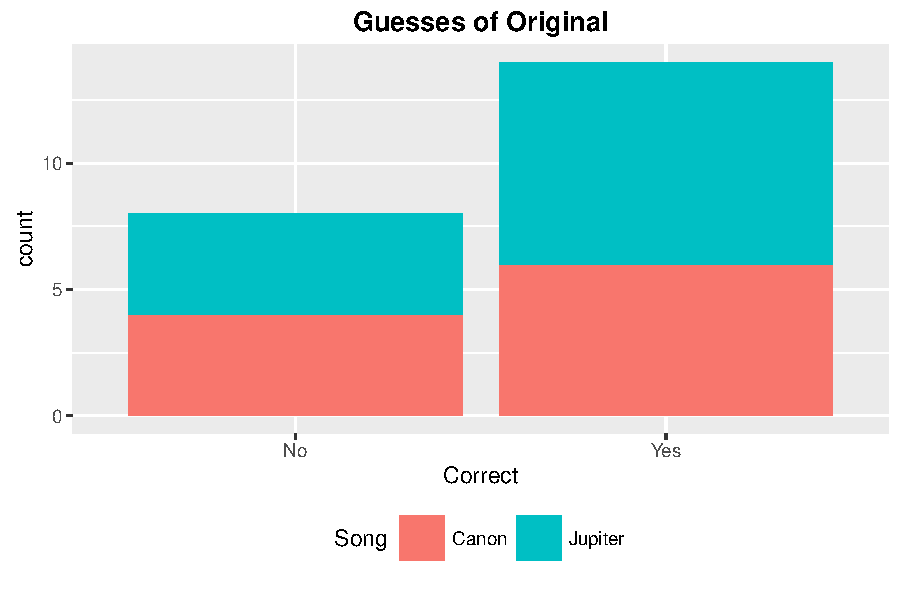
\includegraphics[scale = 0.5]{SurveyGuesses.pdf}
  \caption{Inspiration for the Remixes}
  \label{fig:sub2}
\end{subfigure}
\caption{Survey Results}
\label{fig:test}
\end{figure}




\section{Conclusion and Further Research}

Of the three models used to create the remixed compositions, none of the models produce d pieces that soudned like fundmental music. This is not surprising given the simple structures of our models. There are certain points in soe of the pieces where individual measures sound good, but the overall piece is still not cohesive. The secon order HMM seemed to perform the best in creating music. 

One extension of this project we would like to explore are higher order Hidden Markov Models. Models of higher orders would allow for the current note and velocity to depend on more previous notes. This would introduce more structure and dependence into the models that could create the cohesion in the pieces that was missing before. The second order HMM seemed to perform the best, so it would be exciting to see what a third, fourth or fifth order HMM could do. 

In addition, we need to include the dependencies between the dynamcis and the notes in the model. This could improve the disconerting loud notes in the pieces. Modeling such dependency could also extend to a piece with multiple instruments. This would require the dependencies between instruments to be modeled as well. 

The resulting compositions from these models showed promising results, but there is a lot of room for improvement. The improvements and extensions described above could elevate our results to more cohesive and complicated compositions that have more of a resemblance to music composition. 


\newpage

\section{Appendix}

\subsection{Baum-Welch for Second Order HMM}

1. Run first order Baum-Welch to estimate $\pi$, T, $\phi$. \newline
2. Use second order Baum-Welch to estimate $T_{ijk}$.\newline

Forward Algorithm: \newline
$$\alpha_1(i) = \pi_i \phi_i(x_1)$$
$$\alpha_2(i,j) = \alpha_1(i) T_{ij} \phi_j(x_2)$$
$$:$$
$$:$$
$$\alpha_{t+1}(j, l) = \sum_{i=1}^M \alpha_t(i,j) T_{ijl} \phi_l(x_{t+1})$$
where 2 $\leq$ t $\leq$ T-1 and 1 $\leq$j,k $\leq$ N = M. \newline
Thus, $P(X | \lambda) = \sum_{i=1}^M \alpha_T(i,M)$. \newline

Backward Algorithm: \newline
$$\beta_t(i,j) = \sum_{i=1}^M \beta_{t+1}(j,k) T_{ijk} \phi_k(x_{t+1})$$
where 2 $\leq$ t $\leq$ T-1 and 1 $\leq$ j,k $\leq$ M. \newline

Baum-Welch Estimate for $T_{ijk}$: \newline
$$\beta_t(i,j,k) = \frac{\alpha_t(i,j) T_{ijk} \phi_k(x_{t+1} \beta_{t+1}(j,k)}{P(x|\lambda)}$$ 
where 2 $\leq$ t $\leq$ T-1. \newline

$$\bar{T_{ijk}} = \frac{\sum_t \beta_t (i,j,k)}{\sum_{k,t} \beta_t (i,j,k)}$$

Iterate until $|p_{old} - p_{new}| < tol$. 

\subsection{Baum-Welch for First Order HMM with Two Hidden States}

Define the following:

$$A_{ij} = \textbf{P} (R_t = j | R_{t-1} = i)$$
$$B_{jkl} = \textbf{P} (S_t = l | R_t = j, S_{t-1} = k)$$ 
$$T_{ik, jl} = A_{ij} B_{jkl} = \textbf{P} (R_j = j, S_t = l | R_{t-1} = i, S_{t-1} = k)$$
$$Z_t = (R_t, S_t)$$

The constraints are $\sum_j A_{ij} = 1, \sum_l B_{jkl} = 1.$ \newline

Define c to be a constant. Thus,  \newline
$$Q(\theta, \theta_k) = c + \sum_{t=2}^n \sum_{i,k} \sum_{j,l} \textbf{P}_{\theta_k} (R_{t-1} = i, S_{t-1} = k, R_t = j, S_t = l | x) log T_{ik, jl}$$ 
$$B_{tikjl} = \textbf{P}_{\theta_k} (R_{t-1} = i, S_{t-1} = k, R_t = j, S_t = l | x)$$
$$log T_{ik, jl} = log A_{ij} + log B_{jkl}$$

Thus, \newline
$$ 0 = \frac{\partial}{\partial A_ij}(Q(\theta, \theta_k) - \lambda \sum_{j} A_{ij}) = (\sum_{t=2}^n \sum_k \sum_l B_{tiklj} \frac{1}{A_{ij}}) - \lambda$$
$$\lambda A_{ij} = \sum_{t=2}^n \sum_k \sum_l B_{tikjl}$$
$$\lambda = \sum_j \sum_{t=2}^n \sum_k \sum_l B_{tiklj}$$

For each i, $A_{ij} \propto \sum_{t=2}^n \sum_{k,l} B_{tikjl}$ \newline

$$ 0 = \frac{\partial}{\partial B_{jkl}} (Q(\theta, \theta_k) - \lambda \sum_l B_{jkl}) = \sum_{t=2}^n \sum_i B_{tiklj} \frac{1}{B_{jkl}} - \lambda$$
$$ \lambda B_{jkl} = \sum_{t=2}^n \sum_i B_{tikjl}$$

For each j, k, \newline
$$B_{jkl} \propto \sum_{t=2}^n \sum_i B_{tikjl}$$

\newpage

\section{References}
\begin{enumerate}
\item Wattson, Brett and Ah Chung Tsoi. "Second Order Hidden Markov Models for Speech Recognition", University of Queensland, 146-151. 
\item MIDI Manufacturers Association, "An Introduction to Midi". 
\item Music Composition for Dummies, http://www.dummies.com/how-to/content/music-composition-for-dummies-cheat-sheet.html
\end{enumerate}

\end{document}